\documentclass[10pt,a4paper]{article}
	
	\usepackage{amsmath,amssymb,amsthm,mathtools,amsfonts}
	\usepackage{breqn}
	\usepackage[utf8]{inputenc}
	\usepackage[english]{babel}
	\usepackage[T1]{fontenc}
	\usepackage{graphicx}
	\graphicspath{{../img/}}
	
	%%%%%%%%%%%%%%%%%%%%%%%%%%%%%%%%%%%%%%%%%%%%%%%%%%%%%%%%%%%%%%%%%%%%%%%%%%%%%% Fonts
	
	\usepackage{fontspec}
	\setmainfont{Times New Roman}
	\newfontfamily\garamond[Numbers=OldStyle]{EB Garamond}
	\newfontfamily\plantin[Numbers=OldStyle]{Plantin MT Pro}
	\newfontfamily\wal{Walbaum Com}
	\newfontfamily\quotefont[Ligatures=TeX]{Linux Libertine O}
	\newfontfamily\vest{TRY Vesterbro Regular}
	\newfontfamily\vestb{TRY Vesterbro Poster}
	\newfontfamily\overp{Overpass}
	
	\newfontfamily\mysectionfont[Numbers=OldStyle]{Klavika light}
	
	\usepackage[pdfborder={0 0 0}]{hyperref} %% Ingen firkant rundt om referencer
	\usepackage{multicol}
	\usepackage{tabularx}
	\usepackage{enumitem}% better controls with enumerating
	\usepackage{wrapfig}
		%\setlength{\wrapoverhang}{\marginparwidth}
		%\addtolength{\wrapoverhang}{\marginparsep}
		\setlength{\columnsep}{0pt}
		\setlength{\intextsep}{-10pt}
	\usepackage{caption}
	\usepackage[svgnames]{xcolor}
	\usepackage{dirtytalk}
	\usepackage[modulo]{lineno}
	\usepackage{hyperref}
	\usepackage{pdfpages}
	\usepackage{tasks}
	\newcommand\svar[1]{\newline\textcolor{red}{\textbf{Svar}\\#1}}
	\newcommand{\qm}[1]{“#1”}
	
	%%%%%%%%%%%%%%%%%%%%%%%%%%%%%%%%%%%%%%%%%%%%%%%%%%%%%%%%%%%%%%%%%%%%%%%%%%%%%% Colors
	
	\usepackage{xcolor}
  \usepackage{transparent}
	
	\definecolor{frbblue}{RGB}{47, 88, 109}
	\definecolor{hgred}{RGB}{140, 10, 10}
	\definecolor{frbgreenl}{RGB}{162, 202, 137}
	\definecolor{frbgreen}{RGB}{28, 85, 66}
	\definecolor{frbgrey}{RGB}{243, 245, 242}
	
	
	\usepackage{titlesec}
	\titleformat{\subsection}{\color{frbgreen}\overp\large}{}{}{}
	\newcommand{\source}[1]{Source: \href{#1}{#1}}
	\usepackage{lipsum}
	\usepackage{comment}
	\usepackage{ulem}
	
	%\reversemarginpar
	\newcommand{\glos}[3]{\dotuline{#1}\marginpar{\scriptsize\textit{#3} #2}}

	\setlength{\parskip}{0.5\baselineskip}
	\setlength{\parindent}{0cm}
	\setlist[enumerate]{label=\alph*),left=20pt}
	%\setlist[enumerate]{leftmargin=\parindent}
	%\setlist[enumerate]{nosep}
	
	%Titling
	\usepackage{titling}
	\setlength{\droptitle}{-12ex}
	\pretitle{\begin{center}\vestb\Huge\color{frbgreen}}
	\posttitle{\end{center}}
	\preauthor{\begin{center}\vest\Large\color{frbblue}}
	\postauthor{\end{center}}
	\predate{\begin{center}\vest}
	\postdate{\end{center}}
	
	\setcounter{secnumdepth}{0}
	
	\usepackage{tikz}

\begin{document}

%\pagecolor{FloralWhite}
\title{Eksamen 6l26en}
%\date{\vspace{-5em}} % I tilfældet ingen dato
\date{Sommer, 2026}
\author{Spørgsmål 1}
\maketitle

\begin{tikzpicture}[remember picture,overlay]
    \node[anchor=north east,yshift=-15pt,xshift=-45pt]%
       at (current page.north east)
        {
\includegraphics[scale=0.1]{frbvuc_logo.png}};
    \end{tikzpicture}

\thispagestyle{empty}

\vspace{-4em}

\begin{center}
{\color{frbblue}\rule{1\textwidth}{1pt}}
\end{center}

\subsection{Prøvemateriale}
\begin{description}
\item[Theme:] Voice
\item[Text:] Emma Watson, "Speech on Gender Equality at the UN" (2014) (speech) (abridged)
\item[Instruction:] You must make a presentation (roughly 6 minutes) of the text and relate it to the theme. In your presentation, you must
  \begin{itemize}
\item sum up the main points of the text
\item and make an analysis of the speaker's intention.
\end{itemize}
\end{description}

\subsection{Bedømmelseskriterier, hf C}
Ved den \textbf{mundtlige prøve} lægges der vægt på, at eksaminanden
\begin{itemize}
  \item behersker et forståeligt og sammenhængende engelsk
  \item præsenterer og perspektiverer prøvematerialet
  \item foretager grundlæggende analyse af prøvematerialet med anvendelse af fagets tekstanalytiske grundbegreber
  \item anvender den viden, der er opnået i arbejdet med det studerede emne.
\end{itemize}
Der lægges i bedømmelsen vægt på, at eksaminanden kan indgå i uddybende samtale om præsentationen.

Der gives én karakter ud fra en helhedsvurdering af eksaminandens præstation.


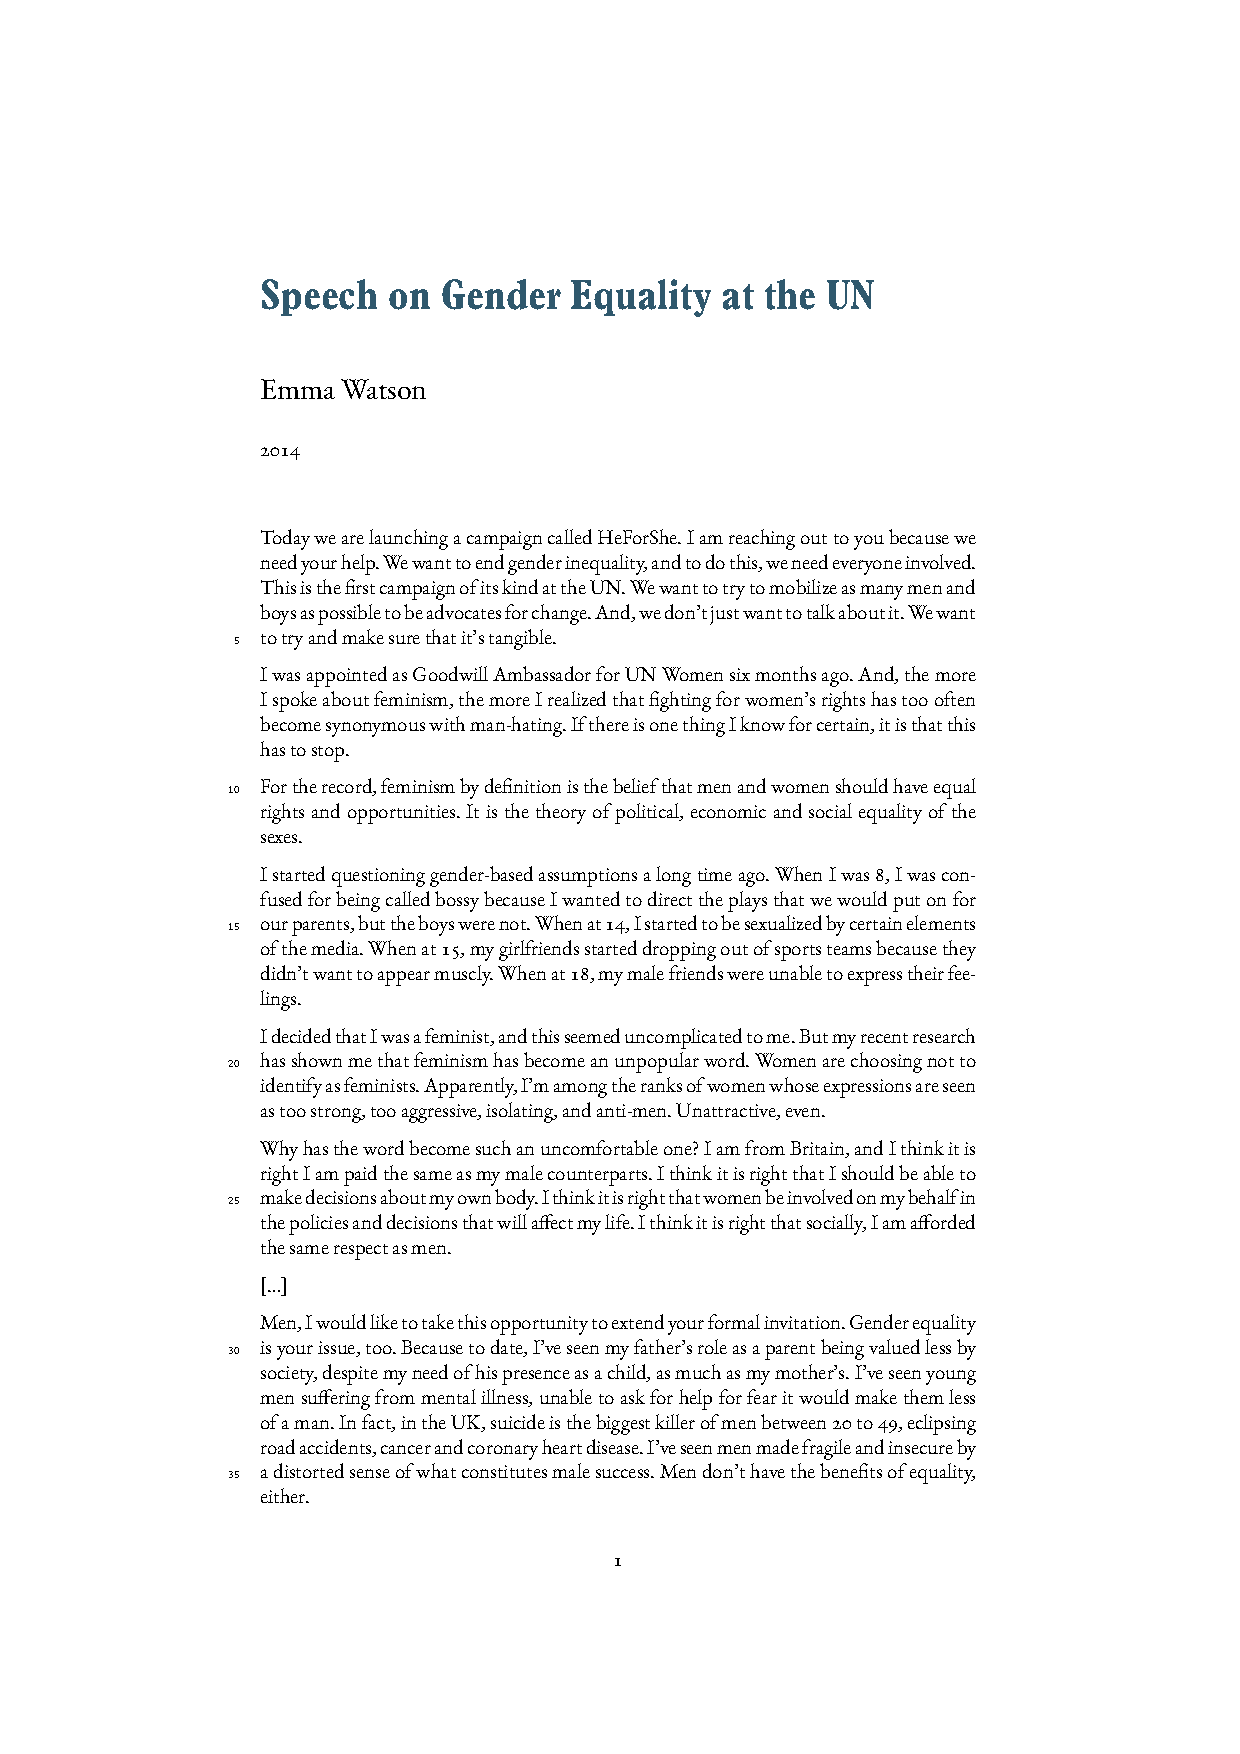
\includepdf[pages=1-]{speech.pdf}






\end{document}


\subsection{Assignment – Short Story (Fiction)}
Write an analytical essay on Haruki Murakami’s short story \qm{On Seeing the 100\% Perfect Girl One Beautiful April Morning}.

Part of your essay must focus on the effect of the short story's preoccupation with dream and reality. It should also include:
\begin{itemize}
\item A \textit{characterisation} of the main character.
\item An intepretation of the short story's \textit{theme} and \textit{message}.
\end{itemize}

Your essay must include references to the short story.


\includepdf[pages=1-]{On Seeing....pdf}

